\documentclass[french]{article}
\usepackage{amssymb, amsmath, mathtools} %pour les mathématiques
\usepackage{fontspec}
\usepackage{xunicode}
\usepackage[a4paper]{geometry}
\usepackage{babel}
\usepackage{hyperref}
\usepackage{pifont}
\usepackage{tikz}
\usepackage{listings}
\usepackage{minted}
\lstset{basicstyle=\ttfamily,
  showstringspaces=false,
  commentstyle=\color{red},
  keywordstyle=\color{blue}
}
\usetikzlibrary{arrows.meta,shapes,positioning,shadows,trees}

\tikzset{
    basic/.style  = {draw, text width=2cm, drop shadow, font=\sffamily, rectangle},
    root/.style   = {basic, rounded corners=2pt, thin, align=center,
                     fill=green!30},
    onode/.style = {basic, thin, align=center, fill=green!60,text width=3cm,},
    tnode/.style = {basic, thin, align=left, fill=pink!60, text width=6.5em},
    edge from parent/.style={->, >={latex}, draw=black, edge from parent fork right}
}

\newcommand{\cmark}{\ding{51}}%
\newcommand{\xmark}{\ding{55}}%

\newtheorem{post}{Postulat}
\newtheorem{mydef}{Définition}

\begin{document}
\title{Résumé Journalier}
\author{Joffrey Hérard}
\date{11 avril 2017} 

\maketitle
\section{Test local avec des conteneurs LXC}
On revient sur les différentes solutions évoqué hier. 
Il est peut être possible de se séparé des solutions tel que Saltstack, au final. Une solution exposé par Phoronix-test-suite, nommé Phoromatic.
Dur notre hôte il est donc nécessaire d'installer le paquet php5-sqlite.
\begin{minted}{bash}
apt-get install php5-sqlite
\end{minted}
On peut considérer cette étapes une fois que phoronix test suite est installe sur tout les invités. 
Toujours sur l'hote on lance la commande suivante :   
\begin{minted}{bash}
phoronix-test-suite start-phoromatic-server
\end{minted}
On a donc un retour 
\begin{minted}{bash}
root@debJo:/home/jo# phoronix-test-suite start-phoromatic-server
Port 8477 chosen as random port for this instance. Change the default port via the Phoronix
 Test Suite user configuration file.
Phoronix Test Suite v7.0.1 (Ringsaker) starting Phoromatic Server
Phoronix Test Suite User-Data Directory Path: /var/lib/phoronix-test-suite/
Phoronix Test Suite Configuration File: /etc/phoronix-test-suite.xml
Phoromatic Server Log File: /var/log/phoromatic.log

Launching with PHP built-in web server.

WebSocket Server Active: localhost:8126
The Phoromatic Web Interface Is Accessible At: http://localhost:8477
\end{minted}
\newpage

\begin{figure}[!h]
Il est important de note le port choisi aléatoirement, vérifier aussi si on peut le changer, au cas ou un firewall empêcherais le bon déroulement de l'application.
L'interface graphique ce présente sous la forme suivante (Image suivante ) : 
\caption{\label{Menu de phoromatic} Menu de phoromatic}
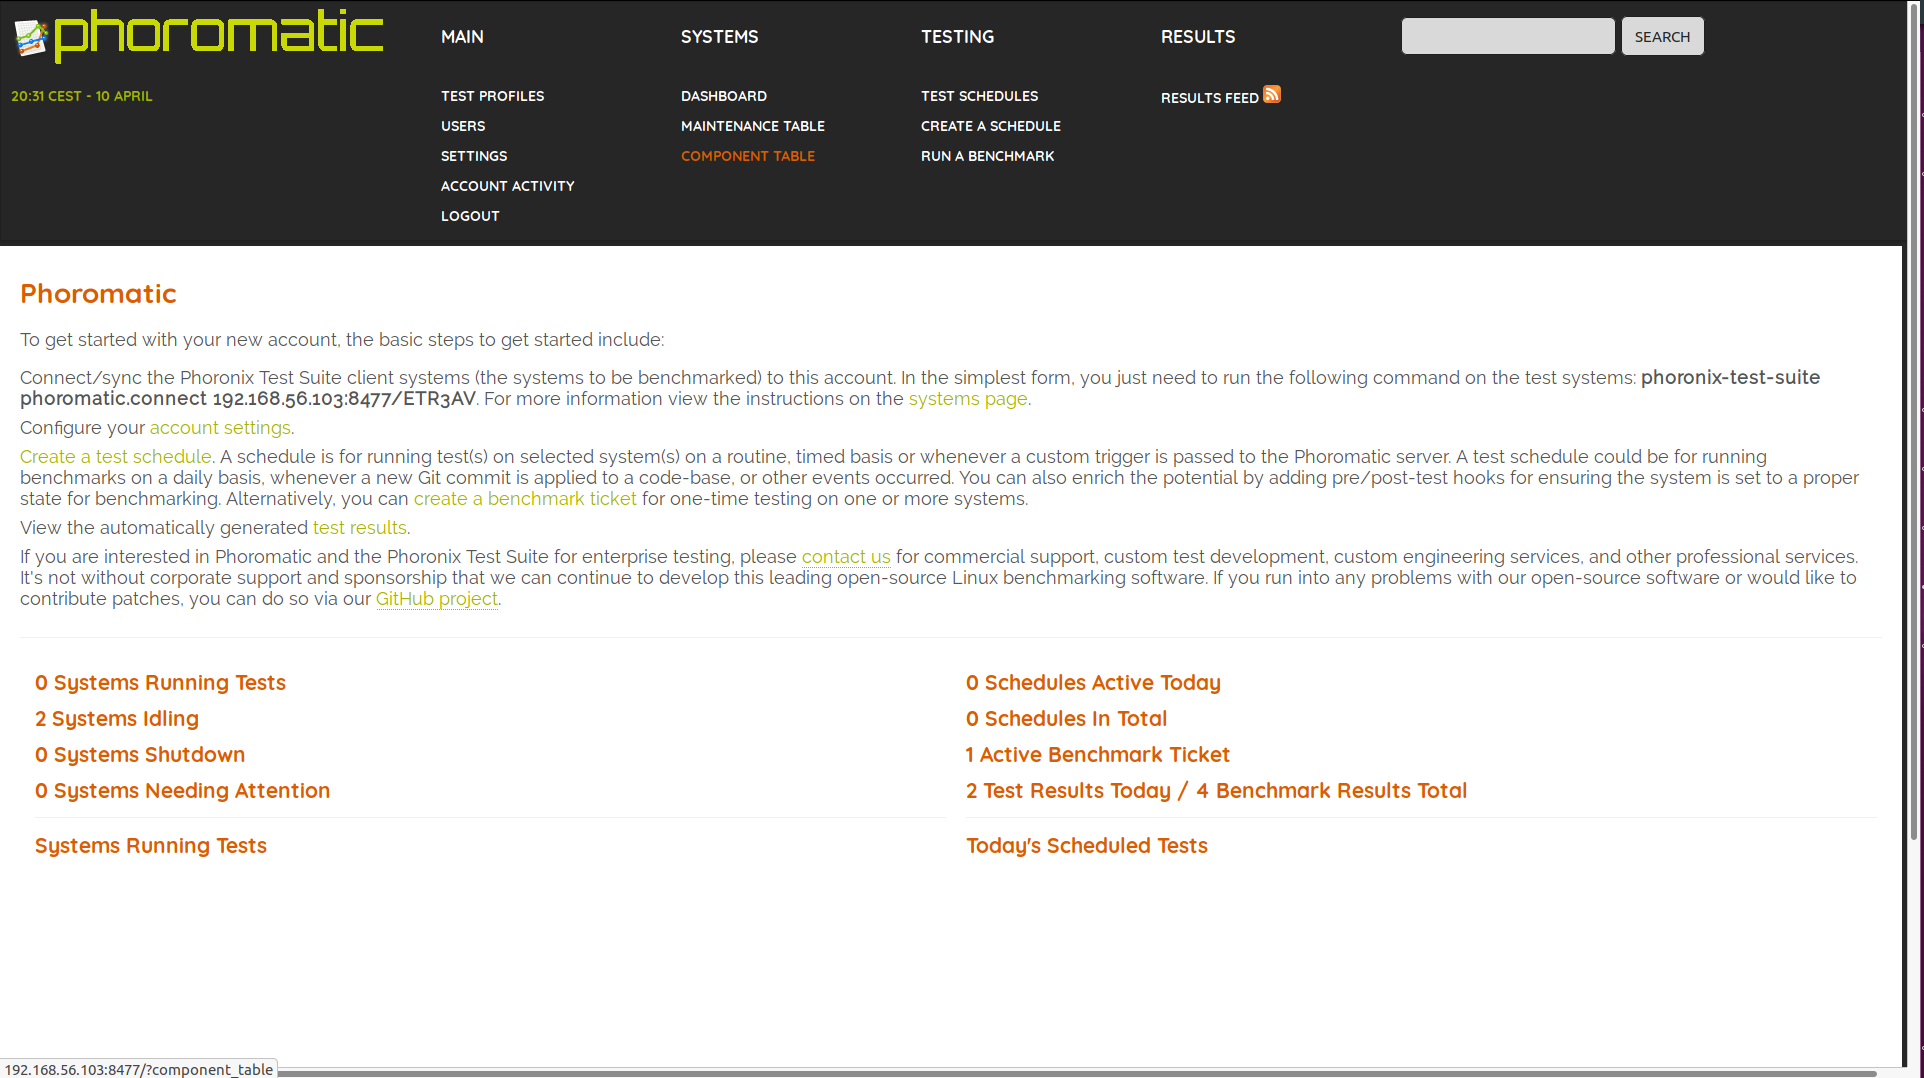
\includegraphics[scale=0.35]{images/menu_phoro.png}
\end{figure} 
\newpage
\begin{figure}[!h]
On constate sur l'image suivante que il y a une machine qui travaille. Auparavant il a fallu l'accepter sur le serveur phoromatic. On est ici d'un point de vu conteneur, et a la fois on a une vue sur le cote serveur du phoromatic donc de L’Hôte.
\caption{\label{ Travail en cours sur L’hôte et l'invite} Travail en cours sur L’hôte et l'invite}
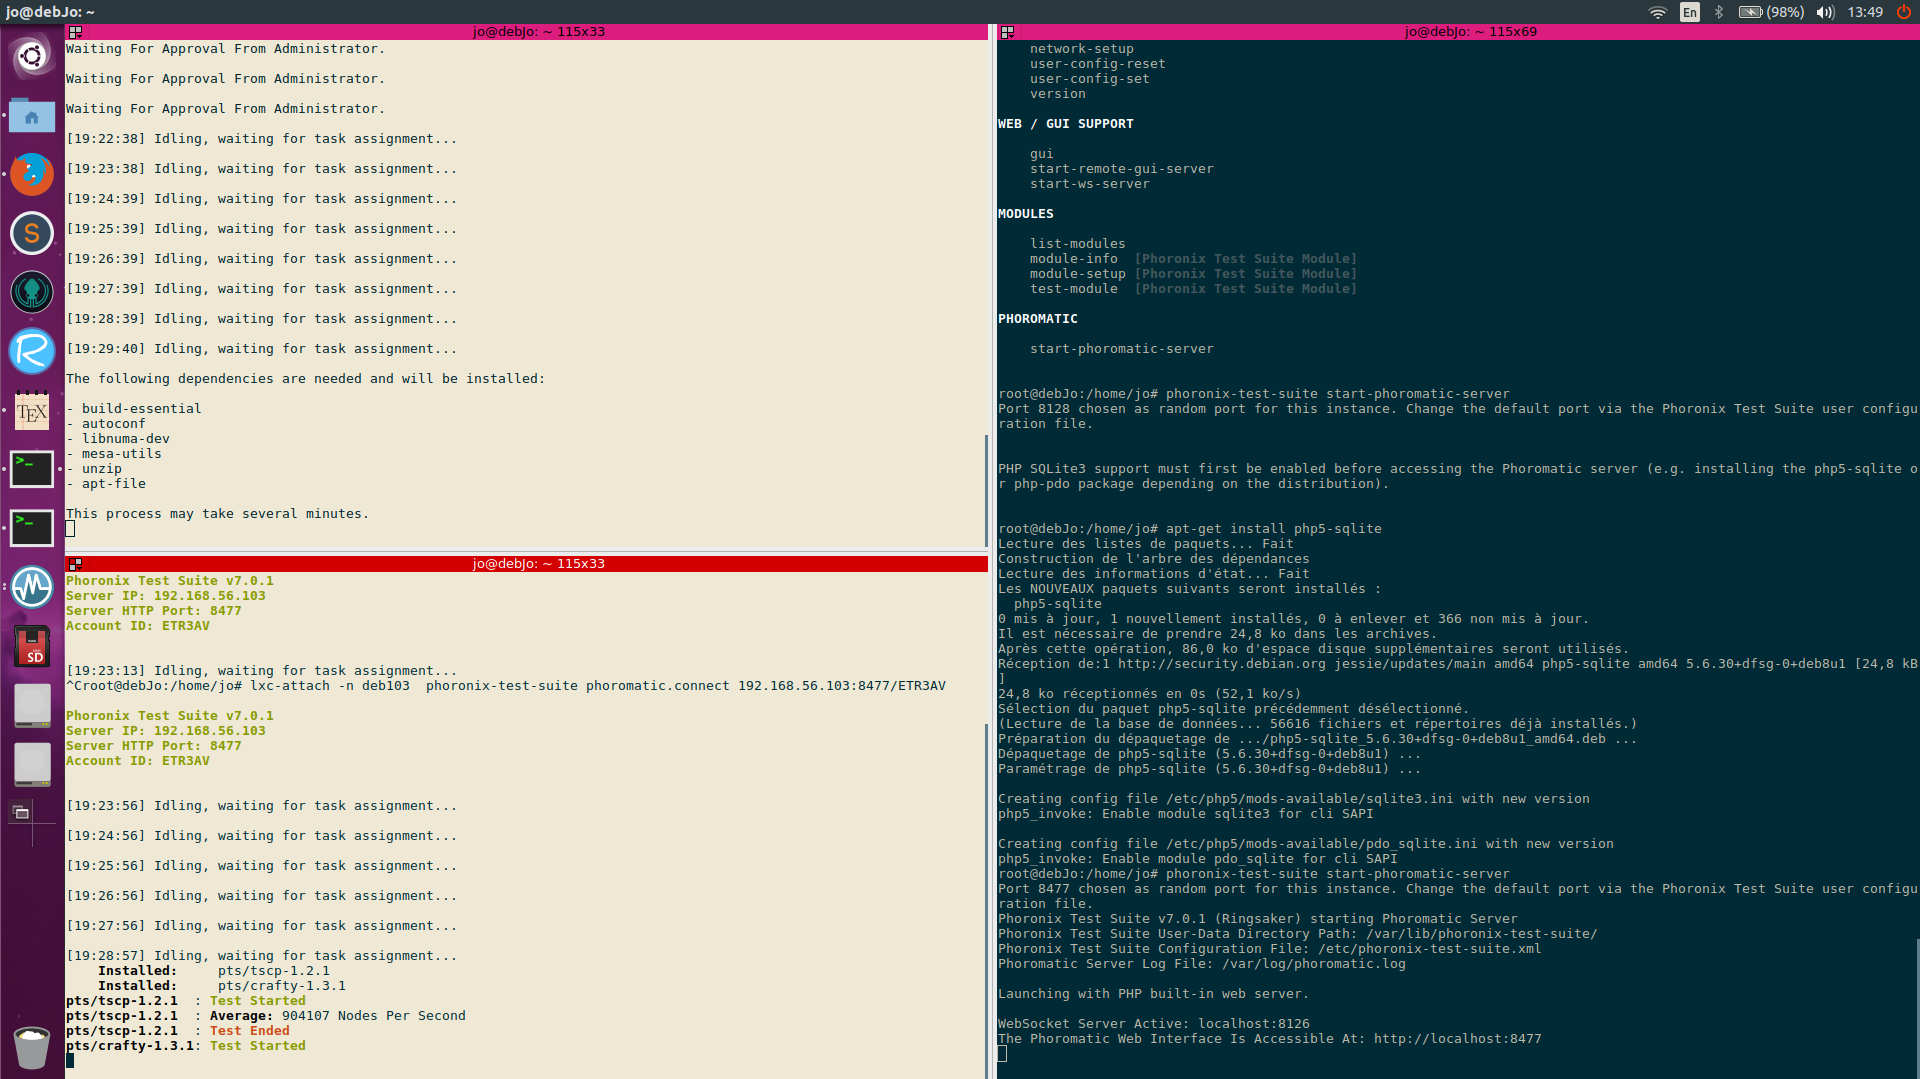
\includegraphics[scale=0.35]{images/capture_phoromatic.png}
\end{figure}
\newpage
\begin{figure}[!h]
Sur cette image on a le retour sur l'interface graphique qu'il y a bel et bien un benchmark/Test qui est en train de se dérouler.
\caption{\label{Information mis a jour sur l'accueil} Information mis a jour sur l'accueil}
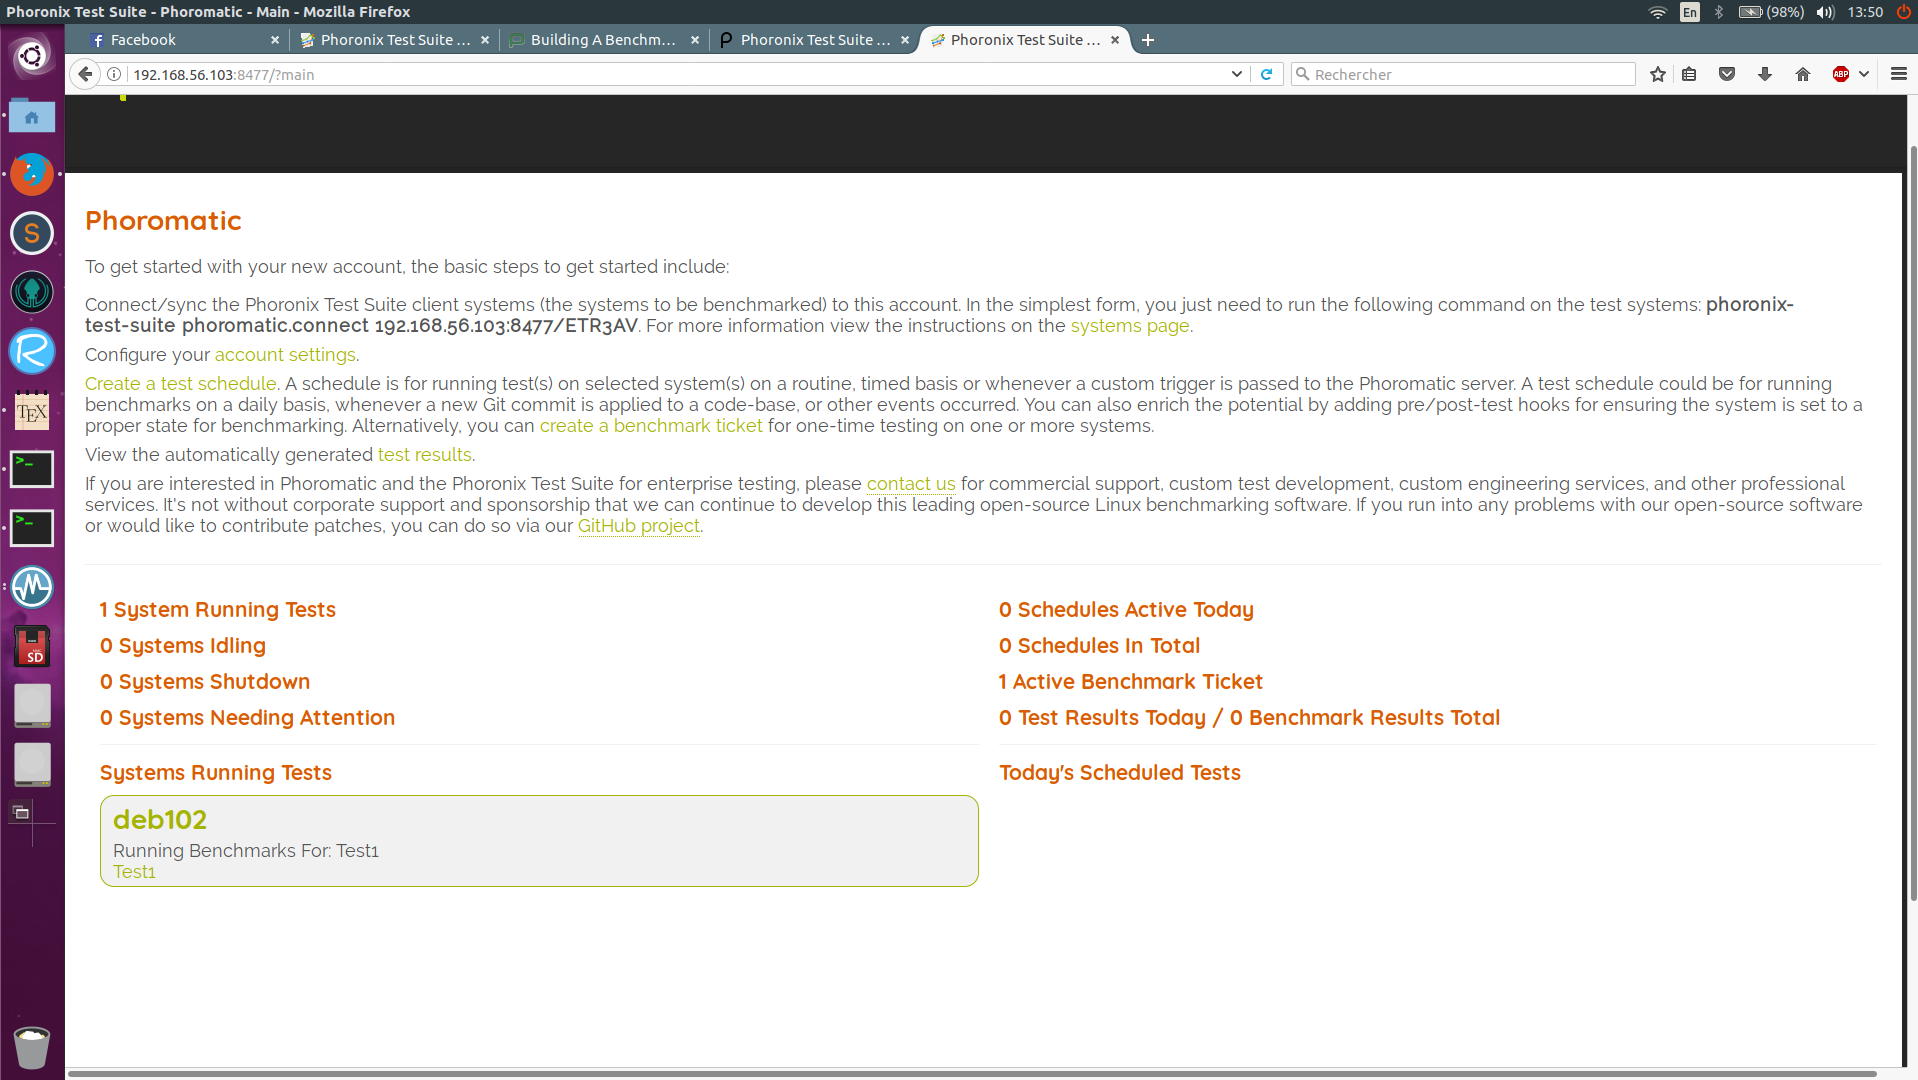
\includegraphics[scale=0.35]{images/debrunningTest.png}
\end{figure}
\newpage
\begin{figure}[!h]
Phoromatic permet de voir les ressources un instant t durant tout le déroulement d'un test.
\caption{\label{Moniteur des ressource de chaque machine} Moniteur des ressources de chaque machine }
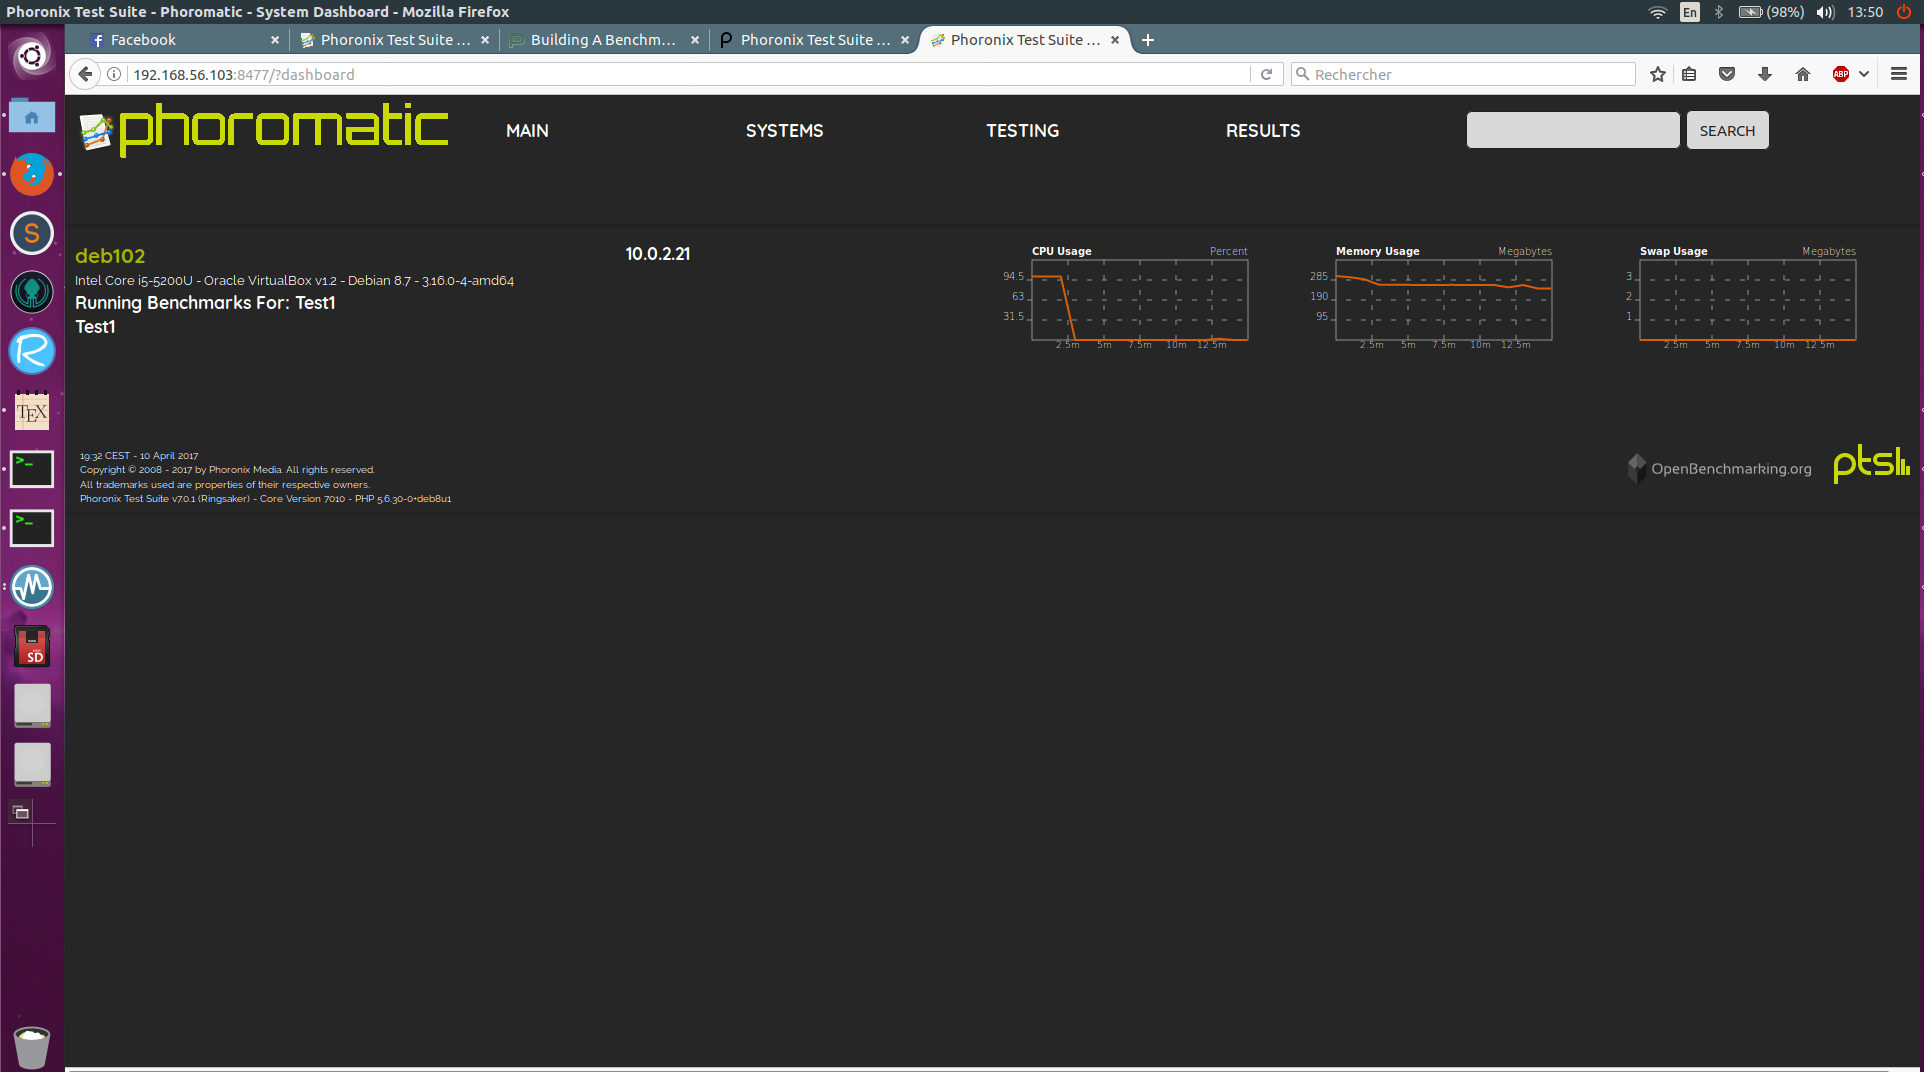
\includegraphics[scale=0.35]{images/monitoring.png}
\end{figure}

\newpage
\subsection{Création d'une suite de tests}
Il est possible avec Phoromatic de faire un enchaînement de plusieurs test d'affiler. On peut choisir, par exemple de faire le programme de test TSCP et crafty qui a été réalise sur les images précédentes pour illustre l'utilisation de l'interface graphique 
Comme l'image le montre :  


\begin{figure}[!h]
On peut donner un titre a notre test un numéro d'identification, c'est aussi 0 cet endroit que l'on sélectionne les machines que l'on veut tester
\caption{\label{Création d'une suite de tests} Création d'une suite de tests}
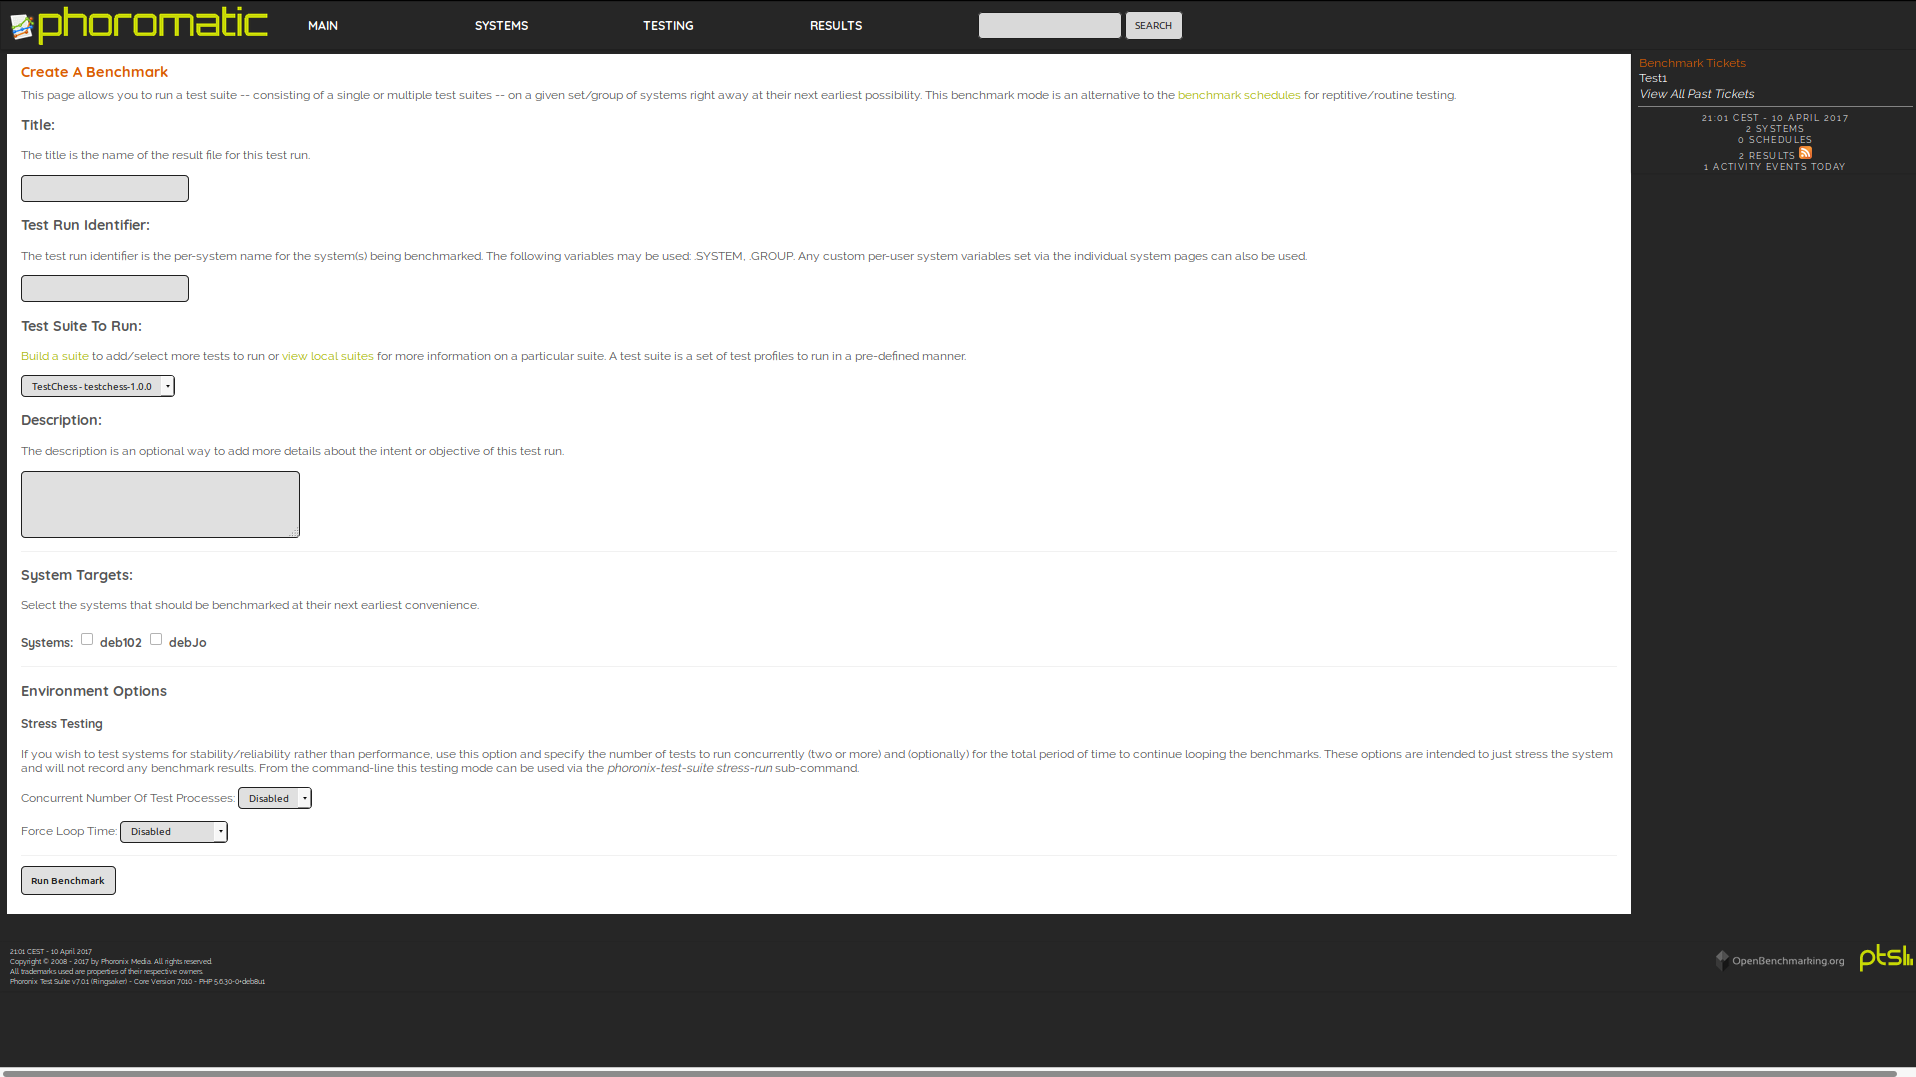
\includegraphics[scale=0.35]{images/createBench.png}
\end{figure}


\newpage
\begin{figure}[!h]
Voici la page de résultats, ainsi on a l'archive de tout les résultats que l'on a eu sur toutes les machines.
\caption{\label{Résultat 2 } Résultat}
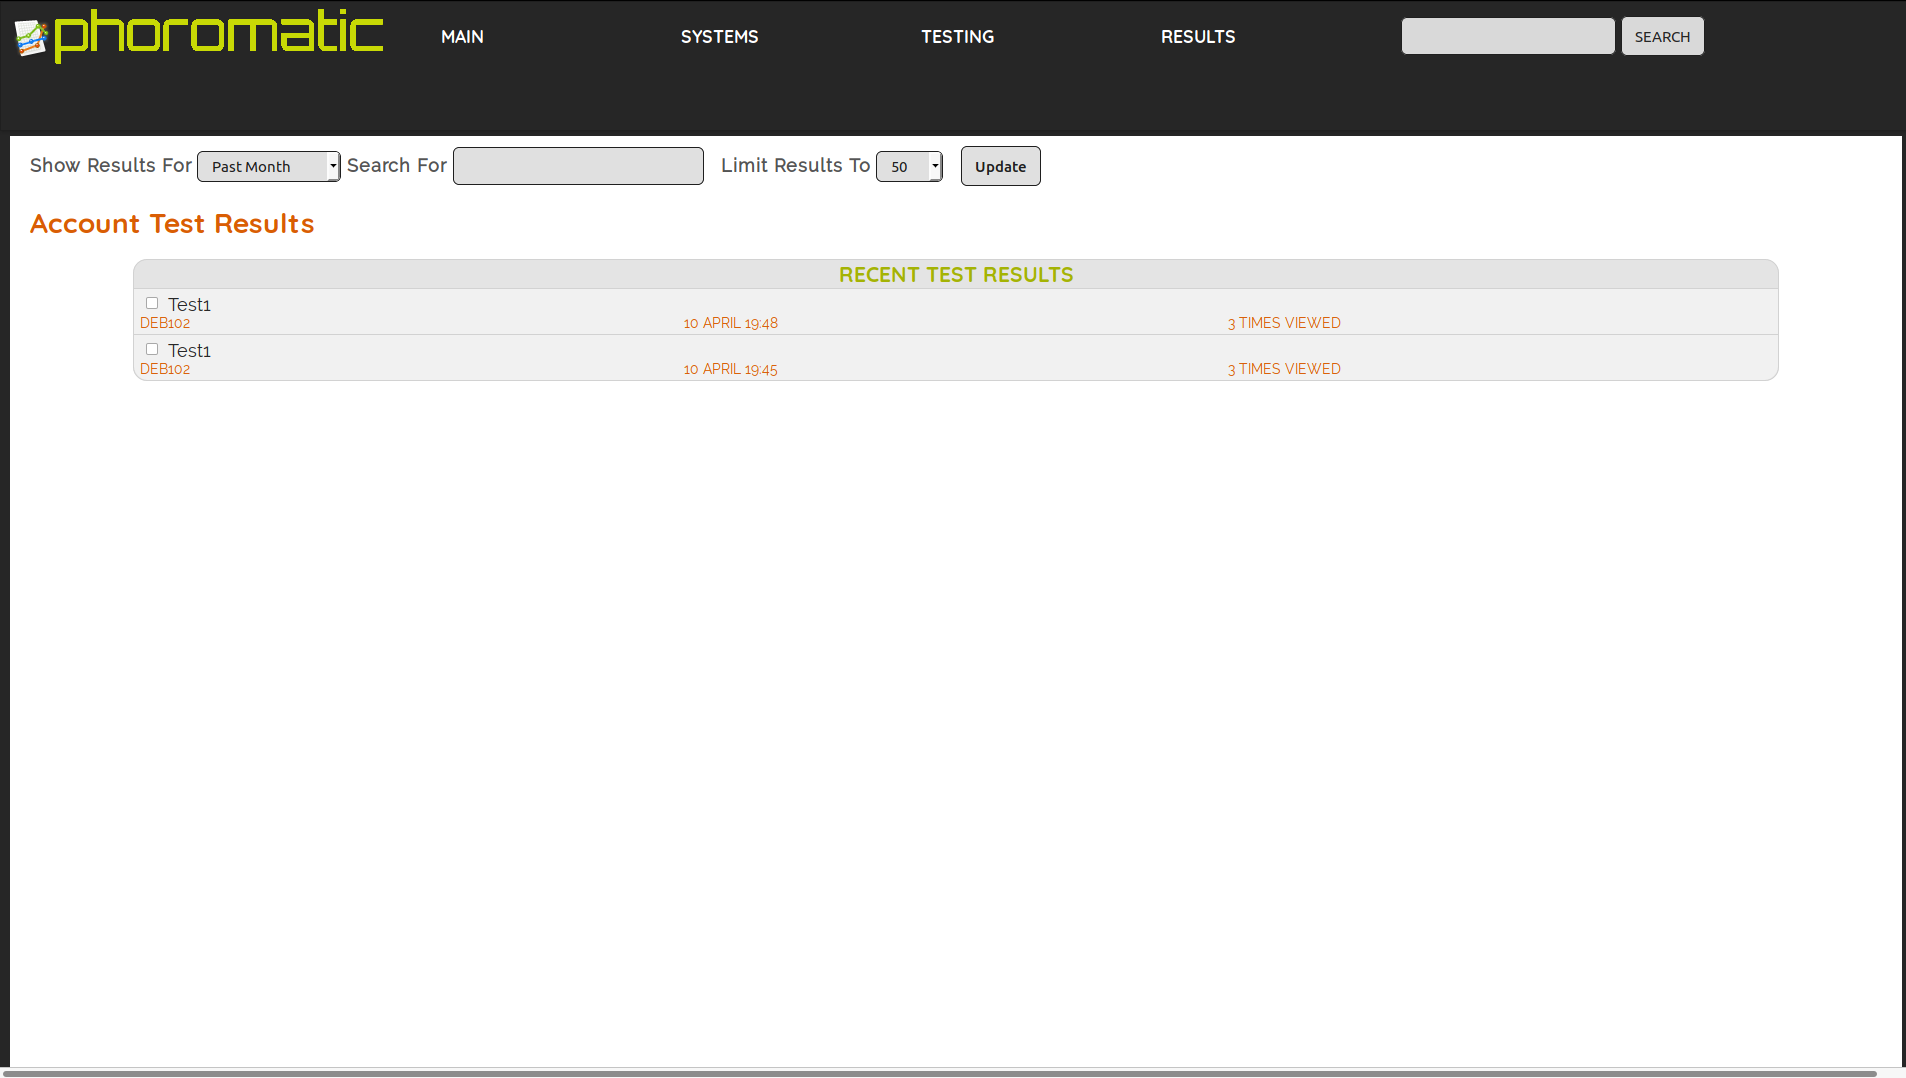
\includegraphics[scale=0.35]{images/res.png}
\end{figure}

\newpage
Voici la page de comparaison des résultats, ainsi on a ensemble de graphique, de resultat chiffre et d'option.
On peut convertir cette page de résultats en 
\begin{itemize}
\item CSV
\item JSON
\item PDF
\item XML
\end{itemize}
On peut aussi normalise les résultats. Pour qu'ils soient plus lisible évidemment. On peut sortir des graphes avec plus de donnée que l'on en a actuellement bien entendu. 

\begin{figure}[!h]
\caption{\label{Résultat} Résultat}
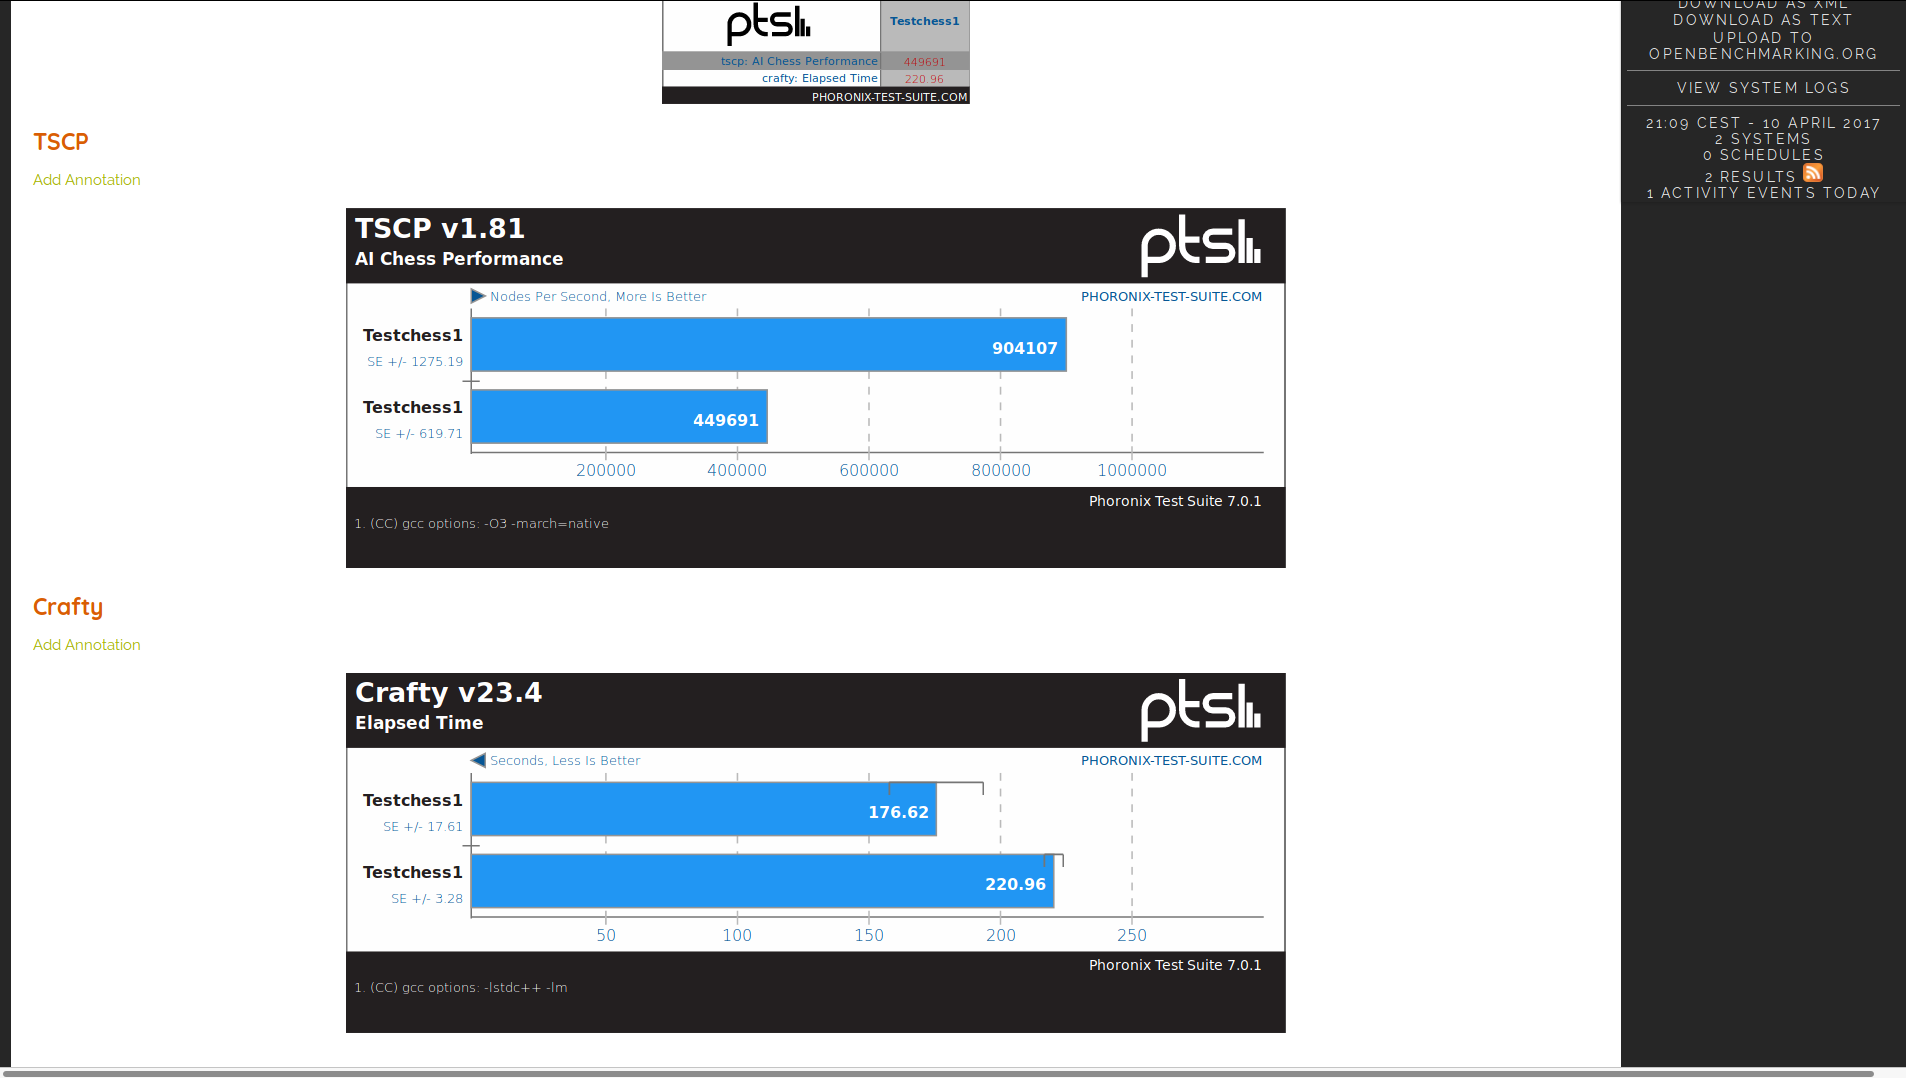
\includegraphics[scale=0.35]{images/res2.png}
\end{figure}

\newpage
\begin{thebibliography}{9}

   \bibitem{Documentation de Phoromatic}
       
          \url{https://www.phoronix-test-suite.com/documentation/phoromatic.html}.

\end{thebibliography}

\end{document}